\section{Method}
\label{section:method}

In this section we describe our method for evaluating the spatial reasoning ability of LLMs, detailing the models and prompts used.


\paragraph{Experimental Setup}
We devise a series of experiments to cover spatial reasoning questions in the form of toponym resolution, and four fundamental spatial relations: metric, directional, topological, and order relationships.

\begin{table}[ht]
    \centering
    \begin{tabular}{l|lrr}
        \textbf{Developer} & \textbf{Model} & \textbf{\#Param} & \textbf{\$ per M/Tok} \\
        \hline
        OpenAI  & gpt-3.5-turbo     & ${\dagger}$ & 00.50/01.50 \\
        ~       & gpt-4             & ${\dagger}$ & 30.00/60.00 \\
        ~       & gpt-4-turbo       & ${\dagger}$ & 10.00/30.00 \\
        ~       & gpt-4o           & ${\dagger}$ & 05.00/15.00 \\
        ~       & ~                 & ~             & ~     \\
        Google  & gemini-1.0-pro    & ${\dagger}$ & 00.50/01.50 \\
        ~       & gemini-1.5-flash  & ${\dagger}$ & 00.35/01.05 \\
        ~       & gemini-1.5-pro    & ${\dagger}$ & 03.50/10.50 \\
        ~       & ~                 & ~             & ~     \\
        Anthropic & claude-3-opus & ${\dagger}$ & 15.00/75.00 \\
        ~       & claude-3-sonnet & ${\dagger}$ & 03.00/15.00 \\
        ~       & claude-3-haiku & ${\dagger}$ & 00.25/01.25 \\
        ~       & ~                         & ~             & ~      \\
        Meta    & llama3-70b        & 70b       & 03.20/03.20 \\
        ~       & llama3-8b         & 8b        & 01.60/01.60 \\
        ~       & ~                         & ~             & ~      \\
        Mistral & mixtral-8x22b-instruct & 39b/141b  & 03.20/03.20 \\
        ~       & mistral-7b-instruct & 7b     & 01.60/01.60 \\
    \end{tabular}
    \caption{Summary of models evaluated.${\dagger}$ denotes where information has not been publicly disclosed.}
    \label{tab:models}
\end{table}

\textbf{Dataset.} 
We develop our own evaluation dataset to reduce the likelihood that the specific questions had been encountered during pre-training by the models under test. 
We select Australia because it is an English-speaking country with place names that are likely to be in the vocabulary of the models, but is less widely documented than places like the Unites States or United Kingdom. 
To reduce the impact of toponym resolution, we use comma groups of \texttt{point/line/region,state} in questions where it doesn't undermine the purpose of the test.
Further, Australia is a large country, with dispersed, dense settlements. 
The population pattern enables us to design tests that combine large and small distances to stress the models under test. 
Importantly, Australia engages in the practice of \textit{dual-naming} locations with their western name and the name given by the traditional owners of the land, allowing us to test using tokens that are less likely to be memorized in geospatial contexts and explore how effectively models encode indigenous history and customs, as it relates to the land.
Our dataset contains $239$ questions that cover the \textit{point, line} and \textit{region} spatial entities as well as the \textit{metric, directional, topological} and \textit{cyclic} relations commonly used in spatial pattern matching.

\textbf{Models.}
We select $14$ models from five of the leading developers of \textit{Large Language Models}. 
We select models that span the available parameter size or self-reported capability where parameters are unavailable, and access them through their Application Programming Interfaces. 
Table~\ref{tab:models} summarizes the selected models, parameters and indicative cost of use. 
For experimentation, temperature is set to $0$ on each model and where available, constant seed values are set to reduce the impact of randomness in generation.

\textbf{Prompting.} 
Each question is provided as an isolated prompt to the model under test so no context is carried between interactions.
We use zero-shot prompting approaches except for where we are shaping the format of the output and in out metric experiments which try to elicit reasoning with in-context learning. 
For each experiment, we begin by providing an initial prompt stating the goal of evaluating spatial reasoning, as follows:

\begin{lstlisting}[title=Prompt 1: Initial System Prompt]
    You are answering to evaluate spatial reasoning ability. You will be presented a question and asked to answer. Where there are multiple possible answers, select the most likely. Answer as briefly as possible, preferring single word answers where they suffice. Where you do not know the answer, it is unanswerable or you are uncertain, return 'ICATQ'.
\end{lstlisting}

\noindent The subsequent prompt is determined by the experiment being conducted.
For each experiment we describe below the specific prompt format used for the second prompt, with letters (A, B, C, etc.) as placeholders for spatial entities such as cities, rivers, roads, and states that we fill in to construct the final prompts.


\subsection{Experiment 1: Toponym Resolution}

\begin{lstlisting}[title=Prompt 2: Toponym Resolution Prompt]
    Where is A? Format your answer as a comma seperated list: state/county, country.
\end{lstlisting}

\noindent We test all points included in the dataset with unaided toponym resolution to identify how strongly each term is associated with Australia, with scoring awarding one point for linking it to Australia, and additional points for more complete comma groups.
We use the results of the toponym experiment (Figure~\ref{fig:toponym}) to filter out terms strongly associated with other countries, (like `Roma' with `Italy' rather than the small town in the Maranoa Region of Queensland) from our subsequent experiments. 
To further reduce the impact of toponym resolution, we use comma groups to specify locations.
Evaluating the toponym tests rewards specificity.
The comma group generated by the model is split and and scored with one point for linking it to `Australia' and additional points for identifying the state and region.

\subsection{Experiment 2: Metric Relations}

\begin{figure}
    \centering
    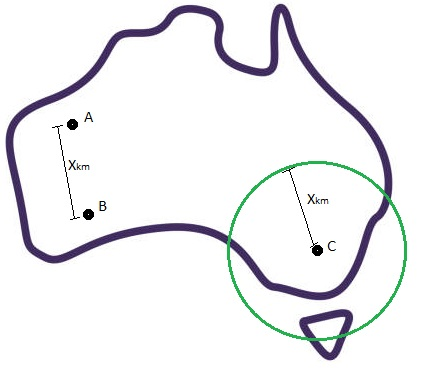
\includegraphics[width=0.3\textwidth]{figures/metric_AUS_diagram.jpg}
    \caption{Visual depiction of the metric relation task corresponding to Prompts 3-5. Given a pair of reference entities $A$ and $B$, and a query entity $C$, the LLM is prompted to retrieve an entity with a metric distance from $C$ as similar as possible to the metric distance between $A$ and $B$. Entities falling on the green circle represent the best responses to the question.}
    \label{fig:metric-AUS-diagram}
\end{figure}

To determine if LLMs can reason about metric (distance) spatial relations, we devise three types of prompts, each asking to retrieve places based on implicit quantitative metric relationships.
%
The general problem is, given a reference pair of cities, $A$ and $B$ that are separated by a distance of $x$, and a query city $C$, the task is to retrieve a fourth city whose distance from $C$ is as close to $x$ as possible.
Since we aim to test for implicit metric reasoning, rather than stating the distance $x$ explicitly, we prompt the LLM for a city whose distance from $C$ is similar to the distance between $A$ and $B$.
The task is depicted visually in Figure \ref{fig:metric-AUS-diagram}, where the ideal response will be the name of a city whose geocoordinates fall on or near the perimeter of the circle.
The following `neutral' prompt is the first of the three variants we use to elicit responses from the models:

\begin{lstlisting}[title=Prompt 3: Neutral Metric Prompt]
    The distance from A to B is similar to the distance from C to what other city or town?
\end{lstlisting}

\noindent Based on previous work~\cite{Bhandari2023}, LLMs have been shown to retrieve places that are closer to a query location when the prompt includes the keyword `near', and retrieve places that are farther from the query location when the keyword `far' is used in the prompt.
To further examine this idea we devise two variants of the neutral metric prompt.
By introducing the keyword `near' or `far' into the prompt, we aim to measure if LLMs have a static representation of those keywords, or if they can adapt the meaning of `near' or `far' based on the scale of the question.
The `near' and `far' prompts are as follows:

\begin{lstlisting}[title=Prompt 4: `Near' Metric Prompt]
    If A is 'near' to B, what is a city or town 'near' to C?
\end{lstlisting}

\begin{lstlisting}[title=Prompt 5: `Far' Metric Prompt]
    If A is 'far' from B, what is a city or town 'far' from C?
\end{lstlisting}



\noindent We populate the prompts with cities and towns of varying populations sampled from across the states and territories of Australia, including both indigenous and western place names.
We measure the geodesic distance between the place returned by the LLM and the query location $C$ and report this as \texttt{predicted{\_}distance}.
In the ideal case, the \texttt{predicted{\_}distance} will match closely to the distance $x$, which we report as the \texttt{target{\_}distance}.
Both distances are normalized by the approximate diameter of the country, so that error tolerance scales with $x$.




\subsection{Experiment 3: Directional Relations}

To determine if LLMs can reason about the spatial relationships between multiple locations, we construct a series of prompts asking about the cardinal directionality between pairs of entities.
We create $42$ queries covering $18$ Australian city and town names of varying population size~\footnote{Ranging from 5,297,089 to 37} into groups of `2-way' and `3-way' constraint problems.
For each group consisting of entities A, B, and C, we construct the following 2-way and 3-way directional prompts: 

\begin{lstlisting}[title=Prompt 6: 2-way Directional Prompt]
    A is north, northeast, northwest, south, southeast, southwest, east, or west of B?
\end{lstlisting}

\begin{lstlisting}[title=Prompt 7: 3-way Directional Prompt]
    A is north, northeast, northwest, south, southeast, southwest, east, or west of B and C?
\end{lstlisting}

\noindent We repeat this for each permutation of A, B, and C, reordering them within the prompt text.
Scoring for directional relations rewards specificity, with more points being awarded for `northwest' rather than `north' or `west' when both could be true. 
% if needed: when wrong response is produce, the geo-coordinates are further included in the prompt.
% if needed: try the reverse where we ask for a city thats SE of A and NW of B
% if needed do more than 3 way and show how accuracy declines with more entities (more complexity)
% Test pairs as baseline? Should be similiar to results MaaSDB got



\subsection{Experiment 4: Topological Relations}
To determine if LLMs can reason about topological relations, we construct a series of seven topological relation prompts containing questions pertaining to each of the major topological predicates.
We select points (P) from a set of city and town names in Australia, regions (R) from a set of lakes, parks, regions, and states in Australia, and lines (L) from a set of highways, roadways, and riverways in Australia.
% Prompts combine the topological predicates with these three spatial entity types
%We construct prompts by selecting 18 pairs of point/line/region entities and assigning each pair a relation from a list of eight standard topological relations: \{\textit{equals, disjoint, intersects, touches, partially overlaps, within, contains}\}~\cite{Carniel2023}.
The prompts are structured as follows:

\begin{lstlisting}[title=Prompts 8-14: Topological Relation Prompts]
    Is A geospatially equal to B?
    Is A geospatially disjoint from B?
    Does A geospatially intersect B?
    Does A geospatially touch B?
    Does A geospatially partially overlap B?
    Is A geospatially within B?
    Does A geospatially contain B?
\end{lstlisting}

\noindent We populate the prompts with cities and towns of varying populations, major waterways, and the `common name' for major roadways (i.e. "The Pacific Highway" rather than "M1 Motorway"). sampled from across the states and territories of Australia, including both indigenous and western place names.
We score the binary response `Yes' or `No' for each answer.
% To understand whether the model was indeed performing spatial reasoning on the topological prompts, we further prompted it with the reverse of some of the prompts.
% For instance, if the original prompt was ``Does R1 meet R2?'' we further prompted with ``Does R2 meet R1?'' and found that in several cases the response was correct for one prompt but not the other.
% These cases indicate that the errors we observe are due to failures in reasoning ability (i.e. that the spatial reasoning the model is doing is not self-consistent) rather than incorrect information about an entity's position in space (such as having false information that a city is located somewhere different from where it actually exists).
% In section \ref{section:future} we discuss data augmentation techniques that may help address the self-consistency issues observed here.

\subsection{Experiment 5: Cyclic Order Relations}
To determine if LLMs can reason about cyclic order relationships, we construct a series of prompts asking about the clockwise or counterclockwise relationship between entities.
%randomly assign nine Australian city names into three groups of three.
For each group consisting of entities A, B, and C, we construct the following prompt: 

\begin{lstlisting}[title=Prompt 15: Cyclic Order Relation Prompt]
    With respect to a centroid in A, is moving from B to C a clockwise or counterclockwise direction?
\end{lstlisting}

\noindent We permute the ordering of A, B, and C, within the prompt text and measure the binary response `clockwise' or `counterclockwise' for each answer.



% \begin{center}
%     \boxed{
%     \!\begin{aligned}
%     & A\ is\ north,\ northeast,\ northwest,\ south,\ southeast,\ \\
%     & southwest,\ east,\ or\ west\ of\ B\ and\ C?
%     \end{aligned}
%     }
% \end{center}







        
% Future Work -------------------------------------

% \subsubsection{E0.1 Non-point Data}
% \paragraph{Method}
% \cite{Liu2023} can do NL2Spatial Query which can handle region/line data, but can an LLM handle it?
% --> Repeat queries similar to \cite{Liu2023} nanjingtest and berlintest region and line queries but instead give them to ChatGPT.
% % randomly pull non-overlapping rivers/highways as lines, lakes, seas, oceans as regions, and landmarks as points and construct directional queries about pairs of them: Lake A is to which side of landmark B


% \nrscomment{Make this a one liner explaining the random selection process and testing to verify it recognizes the cities}
% \nrscomment{move this out to a paper on embeddings}

% \subsubsection{E0.2 Lesser-known Cities}
% To determine if LLMs are able to answer spatial questions about less populous locations and cities, we select 20 Australian city names with varying population sizes and prompt Chat-GPT with the following question, filling in \textit{L} with each city name.

% \begin{center}
%     \boxed{Where\ in\ the\ world\ is\ L?}
% \end{center}

% The locations are selected based on their population size, ranging from 5,297,089 to 37. \nrscomment{fill in details}
% For each prompt, we measure whether the location was recognized or not, and whether the response is spatially accurate or not. 


% \subsubsection{E5. Spatiotemporal and Multiple Hop Relations}
% \paragraph{Method}
% --> Test if Chat-GPT can answer queries like
% - whether event x happened north of event y (2 hops event->loc + loc->spatial)
% - all events in x region that happened between y and z dates (intersect space and time)
% - all events in x region that happened between y and z dates north of location A (spatiotemporal involving spatial relation) 
%\osullikomment{I'd use GDELT data to give you a standard set of events. They're derived from newspaper articles so you should be able to limit to new events and get some confidence that they're not in the training data. Or NewsSTAND I guess....}

%\osullikomment{Could be a really interesting twist using the first nation's territorial boundaries for this as a point of comparison. There are maps out there but they're not well known.}


% \subsection{SPM}
% \nrscomment{Experiment.}
% --> Try giving Chat-GPT a bunch of points A, B, C with coords like the pictorial query grid has and then asking it which cities in a given region match that pattern.
% Also try giving the input instead as a list of pairwise constraints.
% Use OSM to figure out the ground truth by pulling all city tags in the same region and running a traditional SPM algorithm to find all matching patterns.
% Report precision and recall for both input types.

% Check - can it produce an image from the points given? Can we give it an image with points as input?



% \paragraph{Locations being too close to differentiate in the embedding space}
% <ref from translation clustering paper>
% \nrscomment{Experiment.}
% --> Design tests to demonstrate these issues - similar to above, compare the embeddings of locations.